\documentclass{AISB2008}
\usepackage{listings}

\lstset{
  xleftmargin=.35\columnwidth, xrightmargin=.35\columnwidth
}

\usepackage{times}
\usepackage{graphicx}
\usepackage{latexsym}

\usepackage{amsmath}

\makeatletter
\renewcommand{\boxed}[1]{\text{\fboxsep=.2em\fbox{\m@th$\displaystyle#1$}}}
\makeatother

\usepackage{amsopn}
\newcommand{\droparrow}{%
  \mathchoice{\raisebox{-4pt}{$\displaystyle\mapsto$}}
             {\raisebox{-4pt}{$\mapsto$}}
             {\raisebox{-2pt}{$\scriptstyle\mapsto$}}
             {\raisebox{-2pt}{$\scriptscriptstyle\mapsto$}}}

\usepackage{marvosym}


\usepackage[hidelinks]{hyperref}

\begin{document}

\title{The Search for Computational Intelligence,\\ or, How Universal is Universality?}

\author{Joseph Corneli\institute{Department of Computing, Goldsmiths College, University of London\newline\Email \url{j.corneli@gold.ac.uk}} \and Ewen MacLean\institute{School of Informatics, University of Edinburgh\newline\Email \url{ewenmaclean@gmail.com}} }

\maketitle
\bibliographystyle{AISB2008}

\begin{abstract}
XXX YYY
\end{abstract}

\section{Introduction}

\begin{figure}
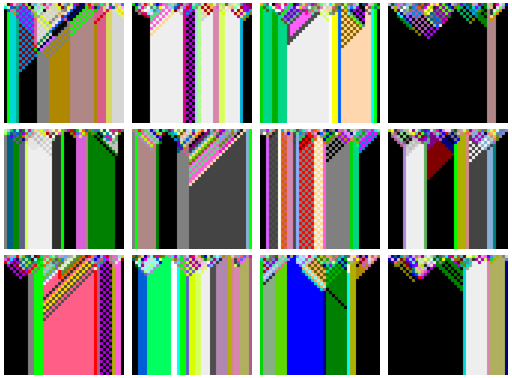
\includegraphics[width=\columnwidth]{metaca.png}
\caption{An illustration of MetaCA evolution}
\end{figure}

This paper takes a local approach to studying the
evolution of cellular automata, following on the
global approach of \cite{pavlic2014self}.

\newpage

\section{Background}

\cite{mitchell1993revisiting} is the classic work on ``edge of
chaos.'' (Read more here and talk about the $\lambda$ thing.)

\cite{hofstadter1995prolegomena,marshall1999metacat} took a rather
different but still somewhat related approach.

\clearpage

\section{Implementation}

To explain how this works, consider the following example.  Each elementary CA rule defines a mapping from all eight strings of 0's and 1's to the set \{0,1\}.  Thus, for example the rule 01010100 is defined as the following operation:
\begin{lstlisting}[mathescape]
0 0 0 $\mapsto$ 0
0 0 1 $\mapsto$ 1
0 1 0 $\mapsto$ 0
1 0 0 $\mapsto$ 1
0 1 1 $\mapsto$ 0
1 0 1 $\mapsto$ 1
1 1 0 $\mapsto$ 0
1 1 1 $\mapsto$ 0
\end{lstlisting}

There are 256 of these rules. So, we can build a CA with 256 colors, rather than the traditional 2, and make the state of any given cell a ``rule''. Then we can apply this rule to decide the output for the next cell, depending on the neighbours. For example, since the middle column in the top half of the diagram below is the rule described above, we can apply this rule to each of the rows in order to produce the result in the bottom half:
\begin{lstlisting}[mathescape]
0 $\mathbf{0}$ 0     $0$ 
1 $\mathbf{1}$ 1     $0$ 
1 $\mathbf{0}$ 0     $1$
0 $\mathbf{1}$ 1  $\droparrow$   $0$
1 $\mathbf{0}$ 0     $1$ 
1 $\mathbf{1}$ 1     $0$ 
1 $\mathbf{0}$ 0     $1$ 
0 $\mathbf{0}$ 1     $1$ 
\end{lstlisting}

This is the straightforward application of a rule without any blending per se, and the results are not particularly impressive.  If we do this with blending, there’s one more step, and we get a different result.

The blending variant says to first compute the ``generic space'' by looking at places where the two adjacent neighbours are the same. Then, whereever we have not resolved the ambiguity (indicated by $\ast$), apply the local rule, as above, to compute the final result: 01101111 in this case.

\lstset{
  xleftmargin=.3\columnwidth, xrightmargin=.3\columnwidth
}

\begin{lstlisting}[mathescape]
0 $\mathbf{0}$ 0     0     $\:0$
1 $\mathbf{1}$ 1     1     $\:1$
1 $\mathbf{0}$ 0     *     $\boxed{1}$
0 $\mathbf{1}$ 1  $\droparrow$   *  $\droparrow$   $\boxed{0}$
1 $\mathbf{0}$ 0     *     $\boxed{1}$
1 $\mathbf{1}$ 1     1     $\:1$
1 $\mathbf{0}$ 0     *     $\boxed{1}$
0 $\mathbf{0}$ 1     *     $\boxed{1}$
\end{lstlisting}

(Say more about Baldwin effect, mutations, and Game of Life
simulator.)

We've put the working code on Github\footnote{\url{https://github.com/holtzermann17/metaca}}. 


\newpage

\begin{figure}
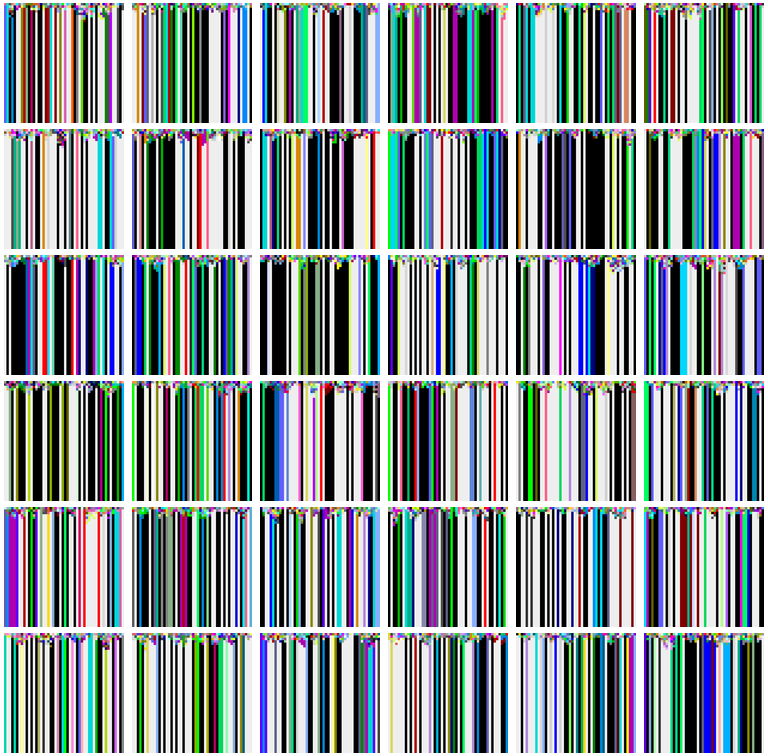
\includegraphics[width=\columnwidth]{paint-drips.png}
\caption{Without the blending rule, things are fairly boring.}
\end{figure}
\clearpage

\section{Results}
(Some pictures can go here).

\begin{figure}

\includegraphics[width=\columnwidth]{flag.png}
\caption{Phenotype with behaviour completely determined by genotype}
\end{figure}

\begin{figure}
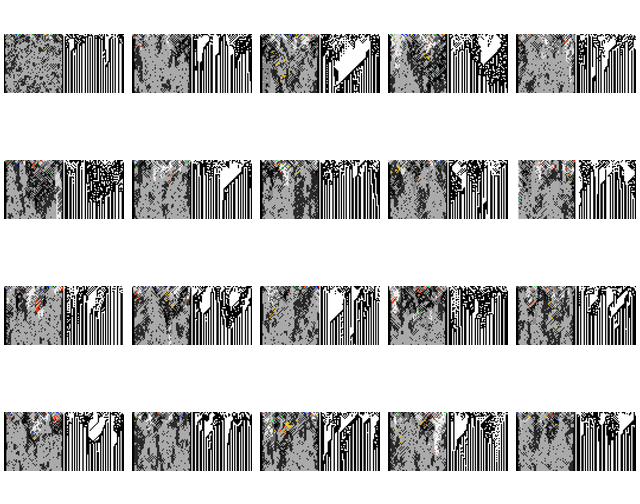
\includegraphics[width=\columnwidth]{baldwin.png}
\caption{Introducing a Baldwin effect}
\end{figure}

\begin{figure}

\includegraphics[width=\columnwidth]{big.png}
\caption{Introducing mutation produces tantalising random structures}
\end{figure}

\begin{figure}
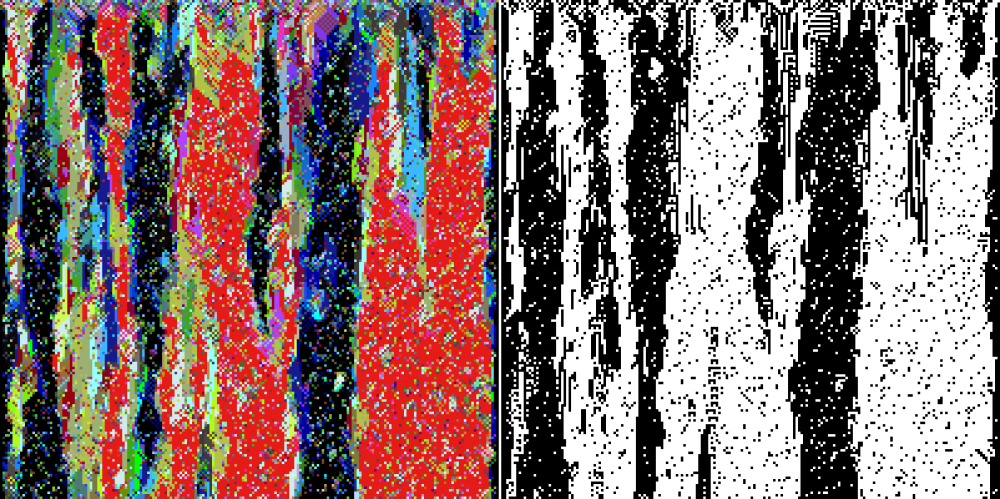
\includegraphics[width=\columnwidth]{lamp-down-low.png}
\caption{Throttling down the mutation rate preserves some of the large-scale stability while making room for variability}
\end{figure}

\begin{figure}
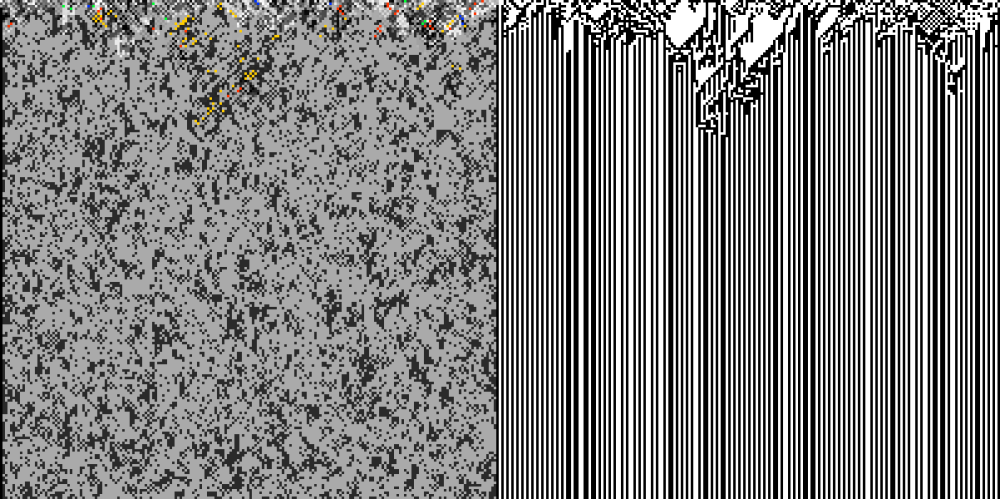
\includegraphics[width=\columnwidth]{eoc.png} \newline
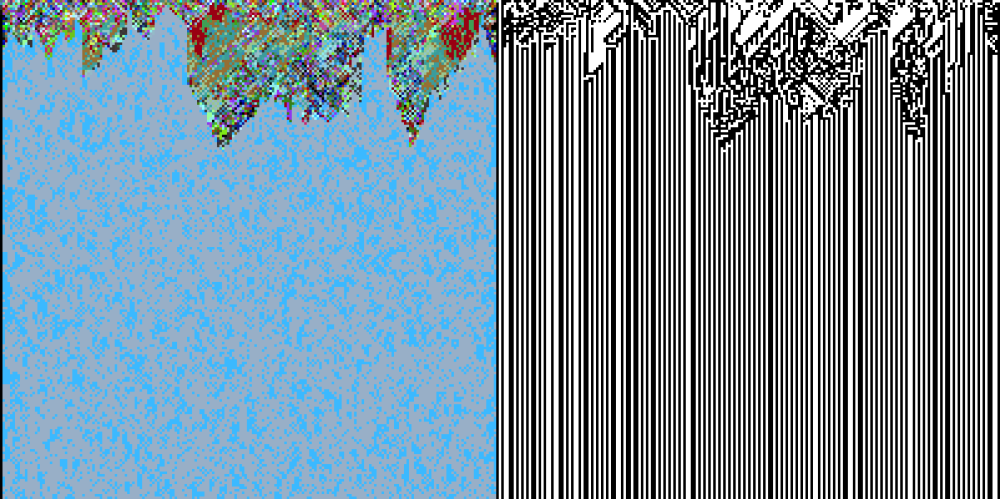
\includegraphics[width=\columnwidth]{reef.png}
\caption{A skewed mutation pattern}
\end{figure}

\begin{figure}
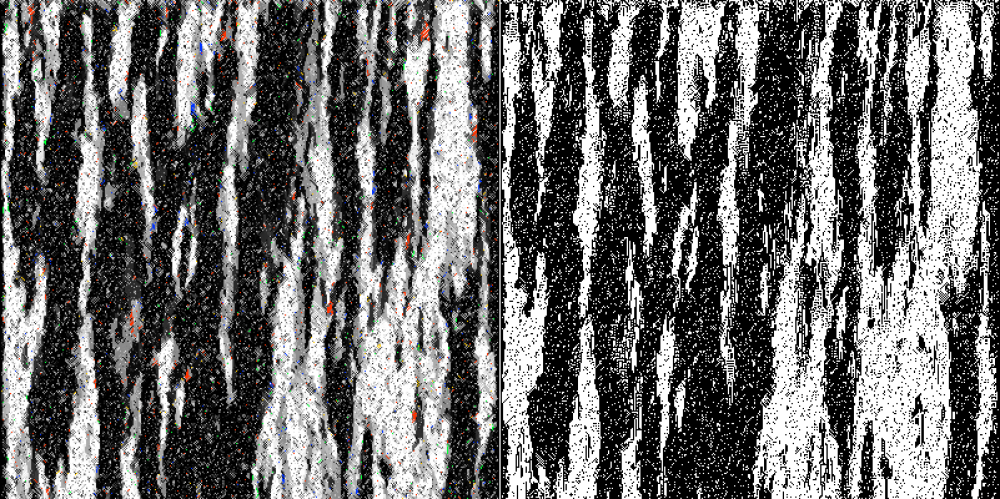
\includegraphics[width=\columnwidth]{seti.png}
\caption{The Search for Intelligent Life in the Universe}
\end{figure}
\clearpage
(Game of life pictures can go here for an interesting comparison
case.)
\newpage

\section{Discussion}

The early experiments seemed provide visual evidence that blending is
a very useful and interesting thing.  Why does it work so well? 

The next set of experiments use a 2-state ``phenotype'' that interacts
with the 256-state ``genotype'' -- or perhaps ``landscape'' or
``ether'' would be a better word.

\clearpage

\section{Conclusion}
% Some of the relevant references are below.
\nocite{*}
We have considerably advanced the field of research.
But much remains to be done.


\section{Acknowledgements}

Coinvent, etc.

\bibliography{metaca}

\end{document}
